\documentclass[english,11pt,a4paper]{article}
\usepackage[T1]{fontenc} % --------------| More characters.
\usepackage[utf8]{inputenc} % -----------| Direct use of scandinavian letters.
\usepackage{float} % --------------------| More options for floats.
\usepackage{graphicx} % -----------------| Support more image formats.
\usepackage{booktabs} % -----------------| Better-looking tables.
\usepackage{tabularx} % -----------------| Better tables
\usepackage{subcaption} % ---------------| Subfigures.
\usepackage[a4paper]{geometry} % --------| Adjusting page margins.
\usepackage{amsmath,amssymb,amsfonts} % -| Various math, including eqref.
\usepackage{xcolor} % -------------------| Allows defn. of custom colors.
\usepackage{babel}
\usepackage{url}
\usepackage{enumitem}

% XY-pic. Used for creating illustrations.
\input xy
\xyoption{all}

% Styling captions.
\usepackage{caption}
\captionsetup{margin=10pt,font=small,labelfont=bf}


%******************************************************************************
% This preabmle contains packages needed to create figures and plots in LaTeX.
%******************************************************************************

\usepackage{etex}
\usepackage{tikz,pgfplots}
\pgfplotsset{compat=1.9}
\usetikzlibrary{calc}
\usetikzlibrary{fit}
\usetikzlibrary{shapes,snakes}
\usetikzlibrary{arrows,decorations.markings}

% Vector Styles for drawings
\tikzstyle{load}   = [ultra thick,-latex]
\tikzstyle{stress} = [-latex]
\tikzstyle{dim}    = [latex-latex]
\tikzstyle{axis}   = [-latex,black!55]


\tikzset{arrowmid/.style={
        decoration={
            markings,
            mark=at position #1 with {\arrow{>}}},postaction={decorate}
    }
}


\tikzset{three sided bottom/.style={
        draw=none,
        append after command={
            [shorten <= -0.5\pgflinewidth]
            ([shift={(-1.5\pgflinewidth,-0.5\pgflinewidth)}]\tikzlastnode.north east) % North edge
        edge([shift={( 0.5\pgflinewidth,-0.5\pgflinewidth)}]\tikzlastnode.north west) % North edge
            ([shift={(-0.5\pgflinewidth,-0.5\pgflinewidth)}]\tikzlastnode.north east) % East edge
        edge([shift={(-0.5\pgflinewidth,-0.0\pgflinewidth)}]\tikzlastnode.south east) % East edge
            ([shift={( 0.5\pgflinewidth,-0.5\pgflinewidth)}]\tikzlastnode.north west) % West edge
        edge([shift={( 0.5\pgflinewidth,+0.5\pgflinewidth)}]\tikzlastnode.south west) % West edge
            % ([shift={( 0.5\pgflinewidth,+0.5\pgflinewidth)}]\tikzlastnode.south west) % South edge
        % edge([shift={(-1.0\pgflinewidth,+0.5\pgflinewidth)}]\tikzlastnode.south east) % South edge

        }
    }
}

\tikzset{three sided top/.style={
        draw=none,
        append after command={
            [shorten <= -0.5\pgflinewidth]
            % ([shift={(-1.5\pgflinewidth,-0.5\pgflinewidth)}]\tikzlastnode.north east) % North edge
        % edge([shift={( 0.5\pgflinewidth,-0.5\pgflinewidth)}]\tikzlastnode.north west) % North edge
            ([shift={(-0.5\pgflinewidth,-0.5\pgflinewidth)}]\tikzlastnode.north east) % East edge
        edge([shift={(-0.5\pgflinewidth,-0.0\pgflinewidth)}]\tikzlastnode.south east) % East edge
            ([shift={( 0.5\pgflinewidth,-0.5\pgflinewidth)}]\tikzlastnode.north west) % West edge
        edge([shift={( 0.5\pgflinewidth,+0.5\pgflinewidth)}]\tikzlastnode.south west) % West edge
            ([shift={( 0.5\pgflinewidth,+0.5\pgflinewidth)}]\tikzlastnode.south west) % South edge
        edge([shift={(-1.0\pgflinewidth,+0.5\pgflinewidth)}]\tikzlastnode.south east) % South edge

        }
    }
}

\tikzset{rectangle split h/.style={
    draw, rectangle split, rectangle split parts=#1, rectangle split horizontal
}}


\tikzset{underbrace/.style={
    thick,
    decoration={
        brace,
        mirror,
    },
    decorate
}}

\tikzset{overbrace/.style={
    thick,
    decoration={
        brace,
    },
    decorate
}}

\tikzset{overbrace label/.style={
    pos=0.5,anchor=south,yshift=0.2cm
}}

\tikzset{underbrace label/.style={
    pos=0.5,anchor=north,yshift=-0.2cm
}}


\geometry{text={.7\paperwidth, .8\paperheight}}

\author{Einar Baumann}
\title{
    \vspace{-1in}
    \usefont{OT1}{bch}{b}{n}
    \vspace{0.1in}
    \rule{\textwidth}{0.5pt} \\[0.5cm]
    \normalfont \normalsize \textsc{TPG4160 Reservoir Simulation} \\ [20pt]
    {\textsc{ \huge Exercise 5 }} \\ [0.5cm]
    {\textsc {\Large Modelling of Horizontal Wells Using ECLIPSE 100} } \\
    \vspace{0.1in}
    \rule{\textwidth}{2pt} \\[0.7cm]
}

\begin{document}
\maketitle
\thispagestyle{empty}
\clearpage

\section{Editing the file} % (fold)
\label{sec:editing_the_file}
For assignment 2, ``9000.00000'' (the reservoir fluid volume rate target/upper limit) in \texttt{WCONPROD} was changed to ``6000.00000'' and ``3000.00000''.

For assignment 3, the entries for $I=2,3,4,5$ were removed from \texttt{COMPDAT} to make the horizontal well shorter.

% section editing_the_file (end)

\section{The effect of changing the production rate} % (fold)
\label{sec:long_}
The base case rates and total production are shown with red lines in Figures \ref{fig:case1}-\ref{fig:case3}. Additionally, they're shown in a combination plot in Figure \ref{fig:combination}.

From Figure~\ref{fig:combination} we see that the rates all start $\approx 1000$ SM3/Day below the number specified in the \texttt{DATA}-file. The rates converge towards the same rate for $Time\gg 0$. We also see that the total production is higher for the runs with a higher reservoir fluid volume rate specified, as would be expected.

% section long_ (end)


\section{The effect of changing the well length} % (fold)
\label{sec:the_effect_of_changing_the_well_length}
As we see in Figures~\ref{fig:case1}-\ref{fig:case3}, shortening the well generally reduces the production rate and total production. This makes perfect sense, as a shorter well implies that the area the fluid can flow through is smaller.

We also see that the impact of shortening the well is smaller for higher production rates. This may be because the effect of increased coning is less pronounced due to the water cut already being quite high for high production rates (see Figure~\ref{fig:watercut}).
% section the_effect_of_changing_the_well_length (end)

\begin{figure}[htbp]
  \centerline{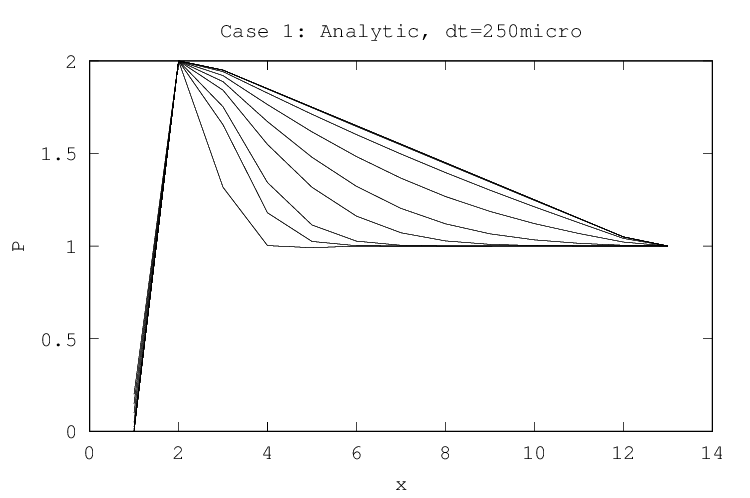
\includegraphics[]{plots/case1.pdf}}
  \caption{}
  \label{fig:case1}
\end{figure}

\begin{figure}[htbp]
  \centerline{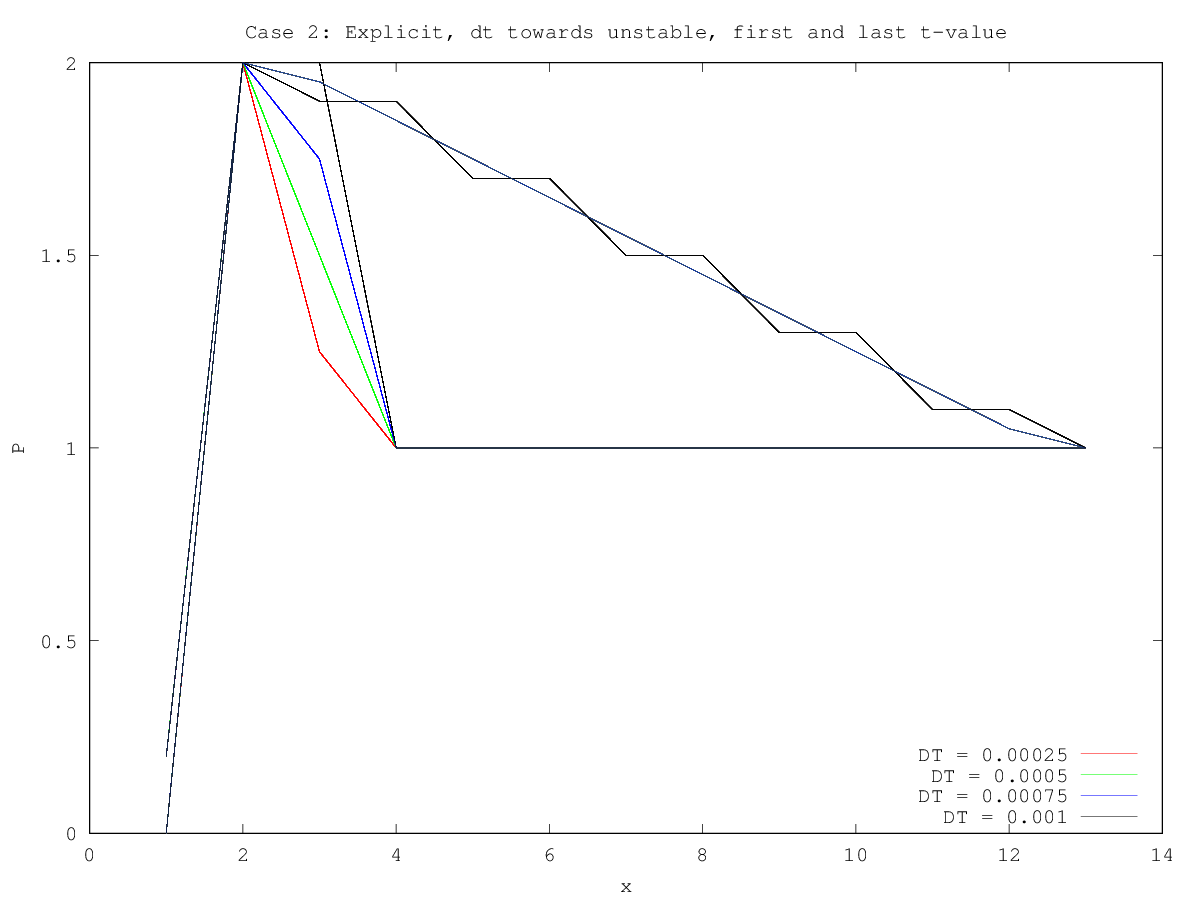
\includegraphics[]{plots/case2.pdf}}
  \caption{}
  \label{fig:case2}
\end{figure}

\begin{figure}[htbp]
  \centerline{\includegraphics[]{plots/case3.pdf}}
  \caption{}
  \label{fig:case3}
\end{figure}

\begin{figure}[htbp]
  \centerline{\includegraphics[]{plots/combined.pdf}}
  \caption{}
  \label{fig:combination}
\end{figure}

\begin{figure}[htbp]
  \centerline{\includegraphics[]{plots/combined_short.pdf}}
  \caption{}
  \label{fig:combination_short}
\end{figure}

\begin{figure}[htbp]
  \centerline{\includegraphics[]{plots/watercut.pdf}}
  \caption{}
  \label{fig:watercut}
\end{figure}

\end{document}
